%%%%%%%%%%%%%%%%%%%%%%%%%%%%%%%%%%%%%%%%%%%%%%%%%%%%%%%%%%%%%%%%%%%%%%%
% Based on IEEE the conference template available                     %
% at https://www.ieee.org/conferences/publishing/templates.html       %
% Adapted for the Data Science Lab course at Politecnico di Torino    %
% by Giuseppe Attanasio, Flavio Giobergia                             %
% 2020, DataBase and Data Mining Group                                %
%%%%%%%%%%%%%%%%%%%%%%%%%%%%%%%%%%%%%%%%%%%%%%%%%%%%%%%%%%%%%%%%%%%%%%%

\documentclass[conference]{IEEEtran}
\usepackage{cite}
\usepackage{amsmath,amssymb,amsfonts}
\usepackage{algorithm}
\usepackage{algorithmic}
\usepackage{graphicx}
\usepackage{textcomp}
\usepackage{xcolor}
\usepackage{subfigure}

\begin{document}

\title{
Lab G7: Natural selection
}

\author{
    \IEEEauthorblockN{Emanuele Pietropaolo}
    \IEEEauthorblockA{
        \textit{Politecnico di Torino} \\
        Student id: s319501 \\
        emanuele.pietropaolo@studenti.polito.it
        }
}

\maketitle
\begin{abstract}
    Natural selection is a key mechanism in evolution, whereby a population evolves due to environmental factors that favour some random mutations over others.
    %
    This paper presents a first approach to simulating such a process over a simplified population. 
    %
    Some assumptions have been made, such as the choice of model and the type of inheritance that the sons will have. 
\end{abstract}

\section{Problem overview}

    In nature, a population starts to evolve because of environmental factors. 
    %
    These factors affect the chances of an individual surviving. 
    %
    There can be many different variables that affect this chance, such as scarcity of resources, predators, disease, etc. 
    %
    Some individuals can develop resistance to one or more of these factors, improving their ability to survive and reproduce, and pass this resistance on to new generations. 

    %1. Introduci una capacità di carico: In natura, l'ambiente ha una capacità di carico massima, che è il numero massimo di individui che l'ambiente può sostenere. Quando la popolazione raggiunge la capacità di carico, la crescita della popolazione rallenta o si ferma. Potresti introdurre un concetto simile nella tua simulazione. Ad esempio, potresti fare in modo che il tasso di riproduzione diminuisca quando la popolazione è vicina alla capacità di carico.

    % 2. Variazione del tasso di riproduzione: Attualmente, tutti gli individui nella tua simulazione hanno lo stesso tasso di riproduzione. In natura, tuttavia, il tasso di riproduzione può variare tra gli individui. Potresti introdurre una certa variazione nel tasso di riproduzione nella tua simulazione. Ad esempio, potresti fare in modo che il tasso di riproduzione di un individuo sia una funzione del suo "lifetime".

    % 3. Mortalità dipendente dalla densità: In natura, la mortalità spesso aumenta con la densità della popolazione. Potresti introdurre un concetto simile nella tua simulazione. Ad esempio, potresti fare in modo che la probabilità che un individuo muoia aumenti quando la popolazione è grande.

    % 4. Riproduzione sessuale: Attualmente, sembra che stai simulando una riproduzione asessuata, in cui ogni individuo produce un figlio da solo. Potresti considerare di simulare la riproduzione sessuale, in cui due individui producono un figlio insieme. Questo potrebbe introdurre ulteriori dinamiche interessanti nella tua simulazione.

\section{Proposed approach}

    Simulating such a complex process can be a challenging task. For this reason, some assumptions have been made:

    \subsection{Assumptions}

    % \begin{figure}[!b]
    %     \centering
    %     \includegraphics[width=\columnwidth]{media/in_p_20_in_lt_2_a_0.01_l_0.5_p_i_0.2/lf.png}
    %     \caption[short]{Lifetime evolution with low $p_i$ and low $\lambda$}
    %     \label{fig:lf_low}
    % \end{figure}

    \begin{itemize}
        \item \textbf{Reproduction:} in nature there are many different forms of reproduction. Most require two individuals of the same species.
        %
        In this simplified version, only asexual reproduction is considered, a form of reproduction that requires a single individual.
        %
        This means that each individual can give birth to
        \item \textbf{Reproduction rate ($\lambda$):} each individual will reproduce with a specified rate of reproduction. In this simplified version, is considered that al the individuals will share the same reproduction rate ($\lambda$) and that this rate is always the same no matter the age of the individual.
        \item \textbf{Reproduction process:} it is assumed that this process follows a Poisson process. In fact, each birth event can be considered as independent and occurring with a given frequency in time. The reproduction process of the whole population can be considered as following a Poisson distribution with a given $\lambda_{tot} = \sum_{0}^{i}\lambda_i$ where $i=$individual. This assumption with the previous one means that the process of the whole population follows a Poisson distribution with $\lambda_{tot} = \lambda \cdot {n}_{pop}$ where ${n}_{pop}=$ size of the population. 
        \item \textbf{Improvement over generation:} this is the process that models how resistance has been passed on to new generations. Each newborn receives a life expectancy from its parents, which is used to generate its lifetime variable. There is a possibility that this lifetime will be greater than the lifetime of the parent ($p_i$). In this case, the lifetime is randomly generated from a uniform distribution between the lifetime of the parent and the lifetime of the parent multiplied by a factor ($1+\alpha$). Otherwise it is generated from a uniform distribution between 0 and the lifetime of the parent.
    \end{itemize}

\section{Results}

    \subsection{Lifetime}

        % \begin{figure}[!ht]
        %     \centering
        %     \includegraphics[width=\columnwidth]{media/in_p_20_in_lt_2_a_0.01_l_1.5_p_i_0.8/lf.png}
        %     \caption[short]{Lifetime evolution with high $p_i$ and low $\lambda$}
        %     \label{fig:lf_grow}
        % \end{figure}

        % In terms of lifetime, we can see in Fig.  that it starts to decrease when the probability of improvement ($p_i$) is low, while in Fig. \ref{fig:lf_grow} it increases otherwise.

    \subsection{Average number of children per generation}
        The average number of children is also an interesting measure, as it also depends on $p_i$.
        %
        % It can be seen in Fig.  that it starts to decrease with a low value of $p_i$, while it remain stable with a high value of $p_i$ (Fig. \ref{fig:av_grow}).

        % \begin{figure}[!ht]
        %     \centering
        %     \includegraphics[width=\columnwidth]{media/in_p_20_in_lt_2_a_0.01_l_0.5_p_i_0.2/av.png}
        %     \caption[short]{Avg. number of children evolution with low $p_i$ and low $\lambda$}
        %     \label{fig:av_low}
        % \end{figure}

        % \begin{figure}[!ht]
        %     \centering
        %     \includegraphics[width=\columnwidth]{media/in_p_20_in_lt_2_a_0.01_l_1.5_p_i_0.8/av.png}
        %     \caption[short]{Avg. number of children evolution with high $p_i$ and low $\lambda$}
        %     \label{fig:av_grow}
        % \end{figure}

    \subsection{Total number of children per generation}

        % \begin{figure}[!ht]
        %     \centering
        %     \includegraphics[width=\columnwidth]{media/in_p_20_in_lt_2_a_0.01_l_1.5_p_i_0.8/tot.png}
        %     \caption[short]{Avg. number of children evolution with high $p_i$ and low $\lambda$}
        %     \label{fig:tot_grow}
        % \end{figure}

        Another interesting measure is the total number of children per generation.
        %
        % In Fig. \ref{fig:tot_low} it can be seen that there is a generation that has given birth to the highest number of children, and this happen in the configuration with the low value of $p_i$.

        % \begin{figure}[!ht]
        %     \centering
        %     \includegraphics[width=\columnwidth]{media/in_p_20_in_lt_2_a_0.01_l_0.5_p_i_0.2/tot.png}
        %     \caption[short]{Avg. number of children evolution with low $p_i$ and low $\lambda$}
        %     \label{fig:tot_low}
        % \end{figure}

        % While Fig. \ref{fig:tot_grow} shows the configuration with an high value of $p_i$ and it can be observed that the total number of children it doesn't show any tendency over time. 
    
\section{Conclusion}

In conclusion, the proposed approach seems to provide some information about the model it wants to simulate. This will serve as baseline for a future approach.

%\bibliography{bibliography}
%\bibliographystyle{ieeetr}

\end{document}
